\section{Prototypen}
\label{prototypen}

Vår prototype, som er vårt forslag til forbedringene vi kom frem til gjennom literaturstudiene, og som ble test gjennom to workshops, er basert på bruk av smarttelefon, i motsettning til telefonene fra cisco som er i bruk i dag. Grunnen til dette valget ligger i at dette er mer fremtidsrettet og gir bedre mulighet for mer utfyllende informasjon i skjermbildet, samtidig som det gir bedre mulighet for interaksjon med brukeren og mulighet for å senere legge til funksjunalitet som eksempelvis å hente frem annen informasjon som blandt annet journaler og prøvesvar. Vi har etterstebet å lage et intuitivt design, som gir god informasjon for å støtte awareness.

\noindent
Applikasjonen er tenkt å være den eneste kjørende på telefonen, hvor vanlige funksjoner som telefon er inkludert, slik at det kun er denne applikasjonen som brukes - også for vanlige telefonsamtaler. Vi vil i de neste delene gi en forklaring på prtotypens design og funksjonalitet.

\subsubsection{Startsiden}
Forsiden er som ilustrert i figur \ref{proto_startside} og med menyvisning som illustrert i \ref{proto_startside_medMeny}.

\begin{figure}[H]
	\centering
	\begin{subfigure}[b]{0.48\textwidth}
		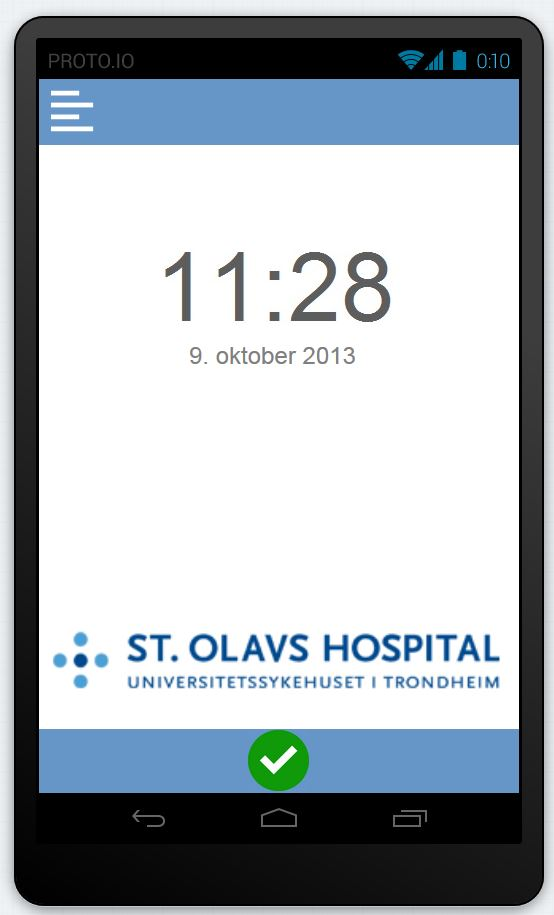
\includegraphics[scale=0.4]{proto_startside.jpg}
		\caption{Prototypens startside}
		\label{proto_startside}
	\end{subfigure}
	\begin{subfigure}[b]{0.48\textwidth}
		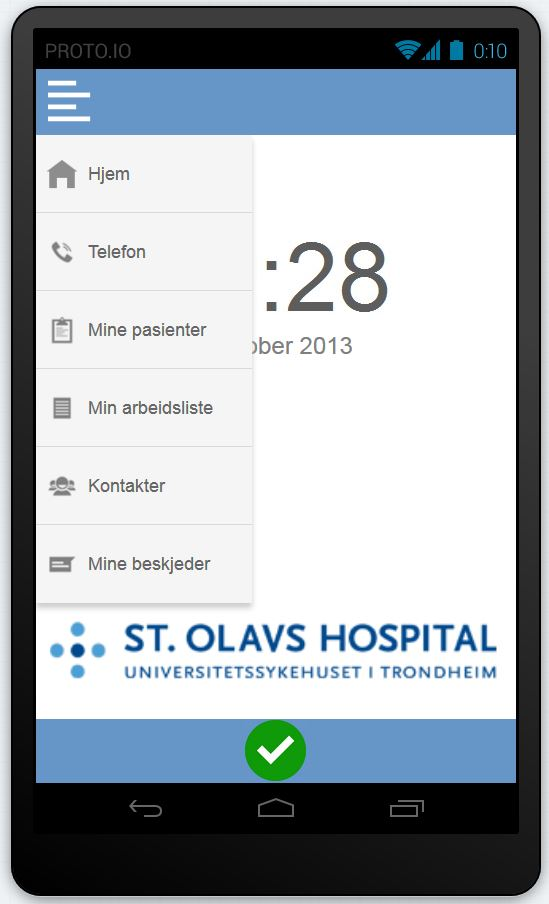
\includegraphics[scale=0.4]{proto_startside_medMeny.jpg}
		\caption{Prototypens startside med menyvisning}
		\label{proto_startside_medMeny}
	\end{subfigure}
	\caption{Prototypens startside}
\end{figure}

\noindent
Forsiden er ment som en standby-side, det vil si at det er denne siden som vises når skjermen slåes på. Tanken var at denne skal være enkel, med få elementer. Vi har derfor valgt ut kun klokken og datovisning i tillegg til status-indikatoren, midt på det nederste blå feltet (her illustrert med en grønn sirkel med hvit hake), og menyknappen øverst til venstre. Status-indikatoren og menyknappen vises på alle skjermbilder, untatt "telefon"\ . 

\subsubsection{Statusindikatoren}
Status-indikatoren har som formål å fortelle sykepleieren om hvilken tilgjengelighetsstatus denne er satt til for øyeblikket. Vi har valgt å bruke tre forskjellige statuser; "tilgjengelig"\ (grønn), "på rom"\ (gul), og "opptatt"\ (rød) (se figur \ref{tilgjengelighetsstatuser}). Denne statusen er i utgangspunktet satt til tilgjengelig. nåe sykepleieren går inn på et pasientrom vil denne automatisk skiftes til på rom , og motsatt når sykepleieren forlater rommet og går ut på gangen/tunet igjen. Teknologien som ligger bak denne automatikken er ikke en del av denne oppgaven. Dersom sykepleieren vet at oppgaven som skal utføres vil ta lang tid, og han/hun helst ikke vil forstyrres i løpet av denne tiden kan statusen manuelt settes til opptatt. Denne statusen vil bli stående til sykepleieren igjen endrer status til tilgjengelig. Eventuelt kan det gis en påminnelse etter en fastsatt tid som spør sykepleieren om det er meningen at statusen fremdeles skal være opptatt, men dette er ikke noe som er implementert i denne prototypen.

\begin{figure}[H]
	\centering
	\begin{subfigure}[b]{0.3\textwidth}
		
\includegraphics[scale=0.15]{statusGronn.jpg}
		\caption{Tilgjengelig}
		\label{proto_startside}
	\end{subfigure}
	\begin{subfigure}[b]{0.3\textwidth}
		
\includegraphics[scale=0.15]{statusGul.jpg}
		\caption{På rom}
		\label{proto_startside}
	\end{subfigure}
	\begin{subfigure}[b]{0.3\textwidth}
		
\includegraphics[scale=0.15]{statusRod.jpg}
		\caption{Opptatt}
		\label{proto_startside_medMeny}
	\end{subfigure}
	\caption{Tilgjengelighetsstatuser}
	\label{tilgjengelighetsstatuser}
\end{figure}

\subsubsection{Pasientsignal}

\begin{figure}
\centering
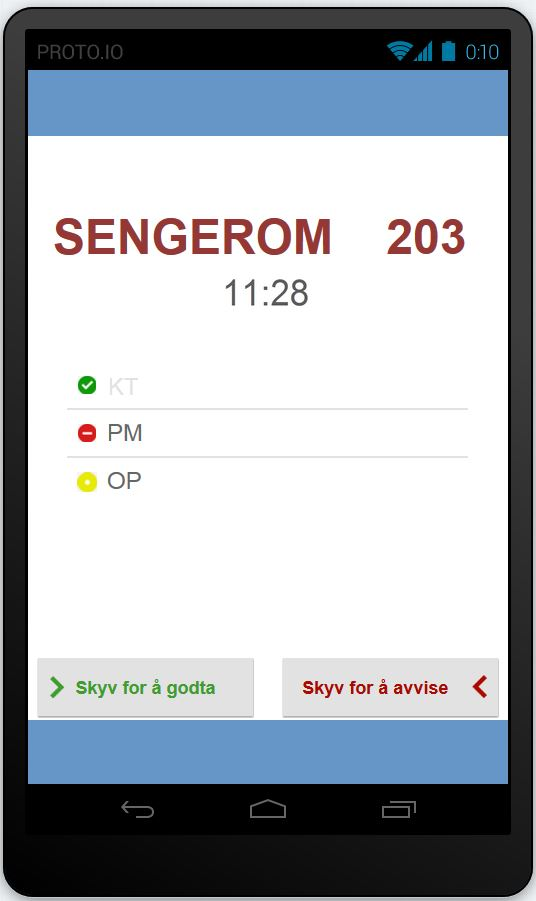
\includegraphics[scale=0.5]{proto_pasientsignal.jpg}
\caption{Skjermbilde ved inkommende pasientsignal. Her fra sengerom 203}
\label{protoPasientsignal}
\end{figure}

Dette er en av de største endringene fra dagens system, og en av hovedfunksjonene med tanke på vår oppgave. Eksempel på enhetene som er i bruk i dag er avbildet i figur [SETT INN REF], mens skjermilde ved pasientanrop ved bruk av prototypen er avbildet i figur \ref{protoPasientsignal}. Den største endringen vi har gjort, borstestt fra design, er at det vises en liste over de neste sykepleierene, samt deres tilgjengelighet, som vil bli oppringt dersom sykepleieren velger i avvise anropet. Hensikten med denne listen er å tilgjengeliggjøre informsjon som kan påvirke sykepleierens avgjørelse i forhold til om anropet skal godtas eller avvises.


